\documentclass{chi-ext}
% Please be sure that you have the dependencies (i.e., additional LaTeX packages) to compile this example.
% See http://personales.upv.es/luileito/chiext/

\copyrightinfo{
  Copyright is held by the author/owner(s).\\
  \emph{CHI'13}, April 27 -- May 2, 2013, Paris, France.\\
  ACM 978-1-XXXX-XXXX-X/XX/XX.\\
}

\title{PaintMobile3D: A Novel Android Application to Draw in 3D}

\numberofauthors{4}
% Notice how author names are alternately typesetted to appear ordered in 2-column format;
% i.e., the first 4 autors on the first column and the other 4 auhors on the second column.
% Actually, it's up to you to strictly adhere to this author notation.
\author{
  \alignauthor{
	\textbf{Nathan Jordan}\\
	\affaddr{University of Nevada, Reno}\\
	\affaddr{1664 North Virginia Street  Reno, NV 89557 USA}\\
	\email{njordan@cse.unr.edu}
  }\alignauthor{
  	\textbf{Halim Cagri Ates}\\
  	\affaddr{University of Nevada, Reno}\\
  	\affaddr{1664 North Virginia Street  Reno, NV 89557 USA}\\
  	\email{cagri@cse.unr.edu} } \\ \\ \\
  \alignauthor{
  	\textbf{Thomas Kelly}\\
  	\affaddr{University of Nevada, Reno}\\
  	\affaddr{1664 North Virginia Street  Reno, NV 89557 USA}\\
  	\email{tjbk123@gmail.com}
  }\alignauthor{
  	\textbf{Sergiu Dascalu}\\
  	\affaddr{University of Nevada, Reno}\\
  	\affaddr{1664 North Virginia Street  Reno, NV 89557 USA}\\
  	\email{dascalus@cse.unr.edu}
  }
}

\teaser{
  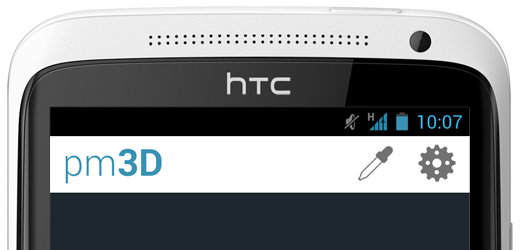
\includegraphics[width=\columnwidth]{teaser2.png}
  \label{fig:teaser}
}

% Paper metadata (use plain text, for PDF inclusion and later re-using, if desired)
\def\plaintitle{PaintMobile3D: A Novel Android Application to Draw in 3D}
\def\plainauthor{Nathan Jordan, Thomas Kelly, Halim Ates, Dr. Sergiu Dascalu}
\def\plainkeywords{smartphones, android, drawing, computer vision }
\def\plaingeneralterms{Design, Algorithms, Human Factors}

\hypersetup{
  % Your metadata go here
  pdftitle={\plaintitle},
  pdfauthor={\plainauthor},  
  pdfkeywords={\plainkeywords},
  pdfsubject={\plaingeneralterms},
  % Quick access to color overriding:
  citecolor=black,
  linkcolor=blue,
  menucolor=black,
  urlcolor=blue,
}

\usepackage{graphicx}   % for EPS use the graphics package instead
\usepackage{balance}    % useful for balancing the last columns
\usepackage{bibspacing} % save vertical space in references
%\usepackage{natbib}

\begin{document}

\maketitle

\begin{abstract} Traditional 3D painting software has relied on building a
two-dimensional representation of three-dimensional space in which the user
can rotate, pan, and zoom. PaintMobile3D takes a different approach. As
smartphones become faster and more feature-rich, we can take advantage of
these improvements to do things that would previously be infeasible. Using a
phone's camera, accelerometer, gyroscope, and/or compass, PaintMobile3D can
track users' movements as they move the phone around in the real world,
allowing them to draw in 3D, based on the motion of the device in the real
world. The user can pick from different colors and can make multiple
``strokes'' using the phone to create more advanced drawings. \end{abstract}

\keywords{\plainkeywords}

\category{H.5.2}{Information interfaces and presentation (e.g., HCI)}{User
Interfaces}. %See \cite{ACMCCS} %See:
%\url{http://www.acm.org/about/class/1998/} %\textcolor{red}{Mandatory section
%to be included in your final version.}

\terms{\plaingeneralterms}

\section{Introduction}

For some time, modeling 3D has been a difficult task due to the problems of
the inherently 2D interaction model provided by computers. By adding a
physical aspect to this, we make it intuitive for users to develop 3D content
quickly and casually. Though there have been other solutions that allow 3D
drawing, the ubiquity of smartphones makes the barrier to entry much lower. A
user can casually decide to waste some time by sketching an object while
waiting for a friend, or perhaps, when seized by a creative fit while out and
about, make a quick sketch of an idea and export it to a common 3D format to
be refined with traditional 3D software.

At its core, PaintMobile3D is about taking the motion of a phone and
translating it into 3D coordinates, used to draw a model. This is done using
the various sensors on modern smartphones: accelerometers, compasses, and
cameras. Newer smartphones also add gyroscopes. Even with all of this data, it
is difficult to keep track of the phone in realtime due to the noisiness of
the signal. Various approaches were combined to create the algorithm used in
this software to maintain the phone's location \cite{voigt2011robust}
\cite{hol2007robust}. However, these approaches used a pre-calibrated camera.
Due to the variation of cameras in phones, we needed to augment this with
Brooks, et al.'s technique for determining egomotion (i.e. the motion of a
camera in an environment) with an uncalibrated camera
\cite{brooks1997determining}.

\section{Copyright}

Copyright (c) 2012, University of Nevada, Reno Department of Computer Science.
All rights reserved.

\pagebreak

\begin{figure} %\hspace*{-0.4\columnwidth}% displace figure
\parbox{1\columnwidth}{

\centering 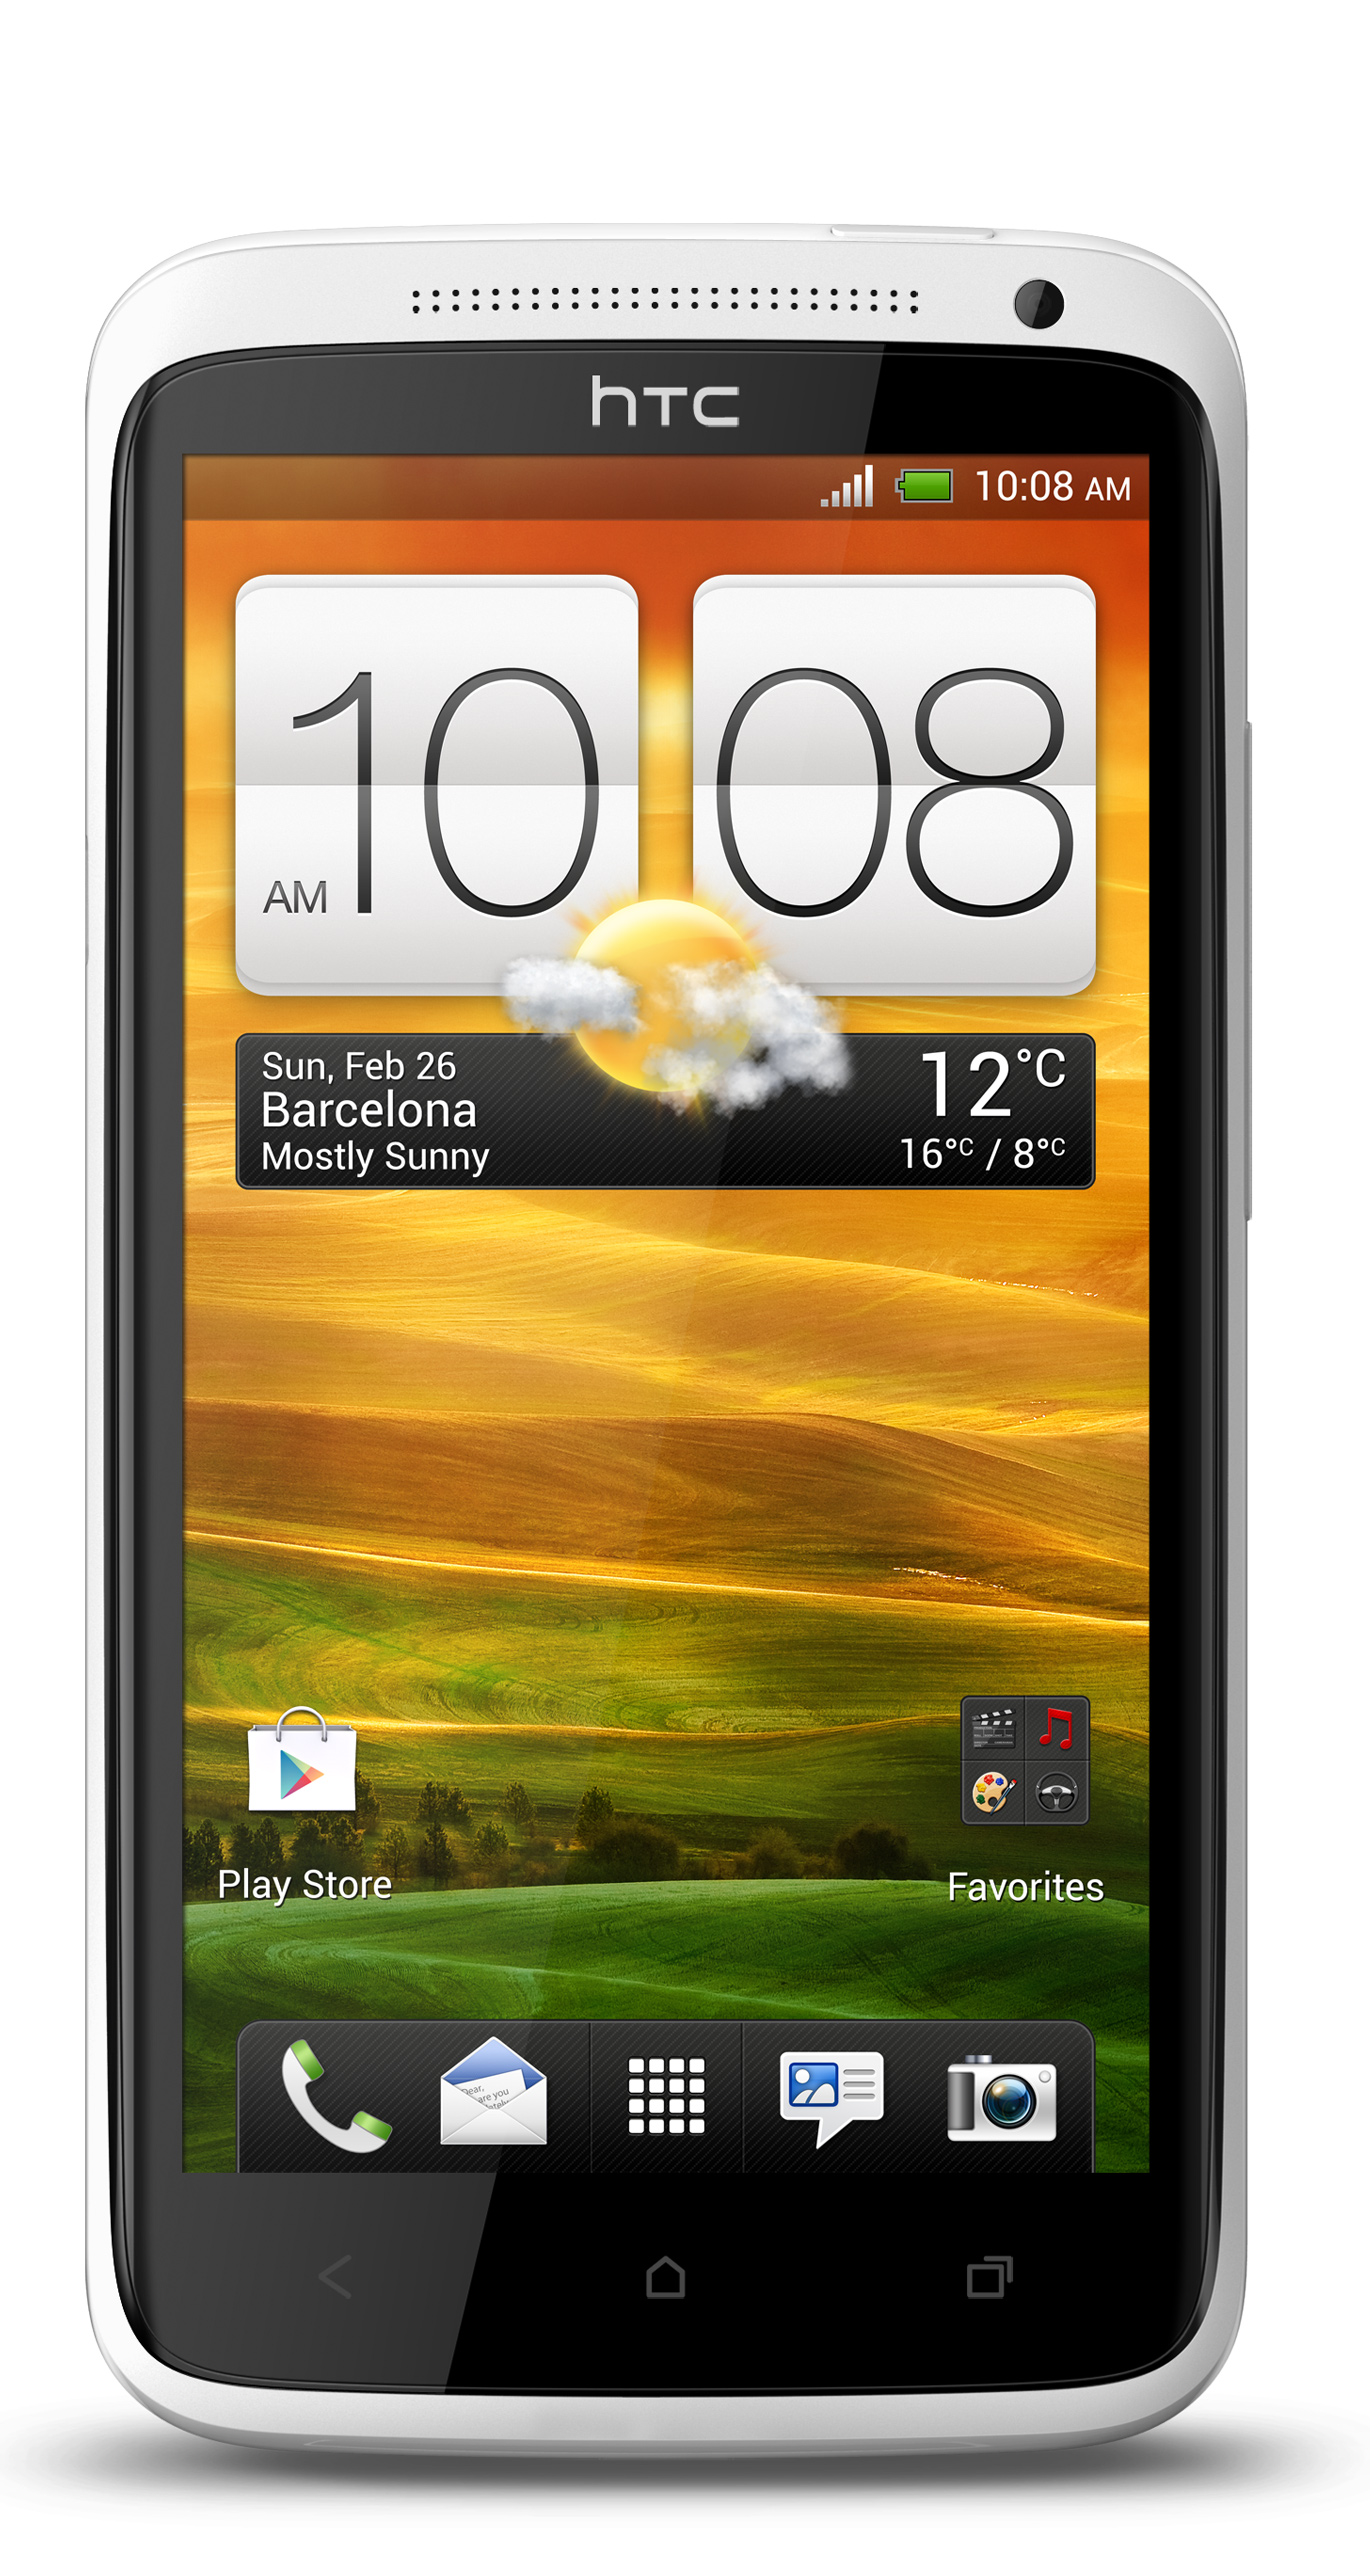
\includegraphics[width=0.8\columnwidth]{onex.jpg} \caption{The main
interface the user is presented with} \label{fig:maininterface} } \end{figure}

\pagebreak

\section{Intended Users \& Usability Goals}

PaintMobile3D is an end-user product that will largely be used for enjoyment.
The application is currently built exclusively for the Android platform, as
such the intended users of the application will be Android smartphone users
with a device running Android 2.3.x (Gingerbread) or newer. The application
currently does not have a specific problem domain outside of entertainment,
and as such can be used by any user without any prior training. PaintMobile3D
requires no configuration for most users, minimal user interface elements (two
options on the ActionBar), and a simple command structure (hold screen to
draw, release to stop drawing). Consequently, PaintMobile3D is a very simple
and easy to use application. Our main goals when creating PaintMobile3D are
the following:

\begin{itemize} \item Create a unique drawing tool for the Android platform
\item Combine the accelerometer, gyroscope and camera data \item Allow the
user to draw by moving their phone through space \end{itemize}

\section{Main Functionality}

The core functionality of PaintMobile3D revolves around the ability to paint
in three-dimensional space. This functionality is provided by combining the
sensor data of the camera of the device, as well as the accelerometer and
gyroscope (if available), which are combined using an algorithm to provide
device localization, that is, the determination of the location of the phone
in a three-dimensional space. We use these measurements to create points in a
virtual coordinate system that can then be used to draw points, lines, or
other geometric shapes. Once the user has drawn his or her object in the
virtual 3D environment, they are free to view the drawing from different
angles and perspectives by orbiting, panning, or zooming the drawing. These
operations are performed by making intuitive gestures on the screen of the
device, such as a swipe to orbit or a pinch to zoom.

\section{Related Systems \& Novelty}

At the time of writing, there are no competing or related systems for drawing
in 3D space using a smartphone. Similar systems exist using camera-based
tracking algorithms to track hand or object movement from a fixed point away
from the user. One such solution takes advantage of the Microsoft Kinect
stereoscopic camera to measure the movement of the user’s hand and deduce 3D
measurements from it to create a single line segment. Another solution
involves instrumentation 

\begin{figure}
%\hspace*{-0.4\columnwidth}% displace figure
\parbox{\columnwidth}{
  \centering
  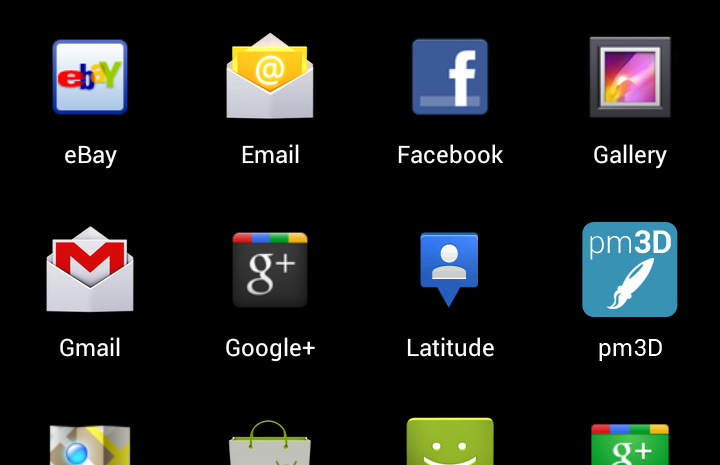
\includegraphics[width=\columnwidth]{icon.jpg}
  \caption{The program is launched via the main Android launcher or a homescreen shortcut}
  \label{fig:icon}
}
\end{figure}

\pagebreak

attached to the users' hand that tracks their
movements and allows them to create strokes in 3D space\cite{schkolne2002drawing}. 
Although these systems allow for tracking an
object in 3D space, they do so using systems that are unavailable on most
smartphones, or do not provide flexibility in regards to location or
portability. PaintMobile3D uses the limited sensory data provided by a modern
smartphone to perform these operations in a multitude of environments and
conditions. The application also provides features like sharing and social
network integration that are unavailable on these related systems. Given the
growing ubiquity of smartphones and social media outlets like Facebook,
Twitter, and Instagram, PaintMobile3D could create a new class of social
interaction with 3D art.

%\begin{figure}
%\hspace*{-0.4\columnwidth}% displace figure
%\parbox{1.4\columnwidth}{
%  \centering
%  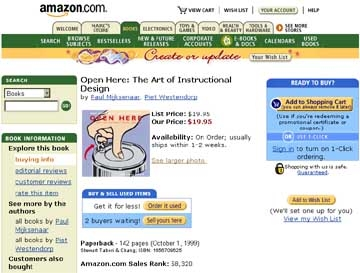
\includegraphics[width=1.4\columnwidth]{sample.jpg}
%  \caption{Insert a caption below each figure. Images can "float" around body text, like this example.}
%  \label{fig:sample}
%}
%\end{figure}

\section{User Interface}

PaintMobile 3D is designed to conform to the Android design guidelines. While the application is compatible with Android 2.3.x (Gingerbread), its targeted version is Android 4.1.x (Ice Cream Sandwich). Thus the application follows the Ice Cream Sandwich design guidelines. The application currently has two main screens or "activities", the main screen and settings screen. The settings screen contains options to change which sensors are used in the localization algorithm, calibrating sensors, as well as information about the application and the developers. The main application interface includes an ActionBar (a standard Android design convention), which takes all the important functionality of the application and keeps it readily available for the user to access. In PaintMobile3D, these actions include accessing the settings page, changing the color of the drawing, and extra options such as sharing, loading, and saving the drawing. The bulk of the main interface is taken up by the drawing area. After the user draws the shape by moving the phone around. the drawing that is computed based on these motions is shown in this area. The user can pinch the screen to zoom in or out, and swipe the screen to orbit. We chose not to allow the user to translate, as they may get lost in the environment and would degrade user experience. 

\begin{figure}
\hspace{\columnwidth}% displace figure
\parbox{\columnwidth}{
  \centering
  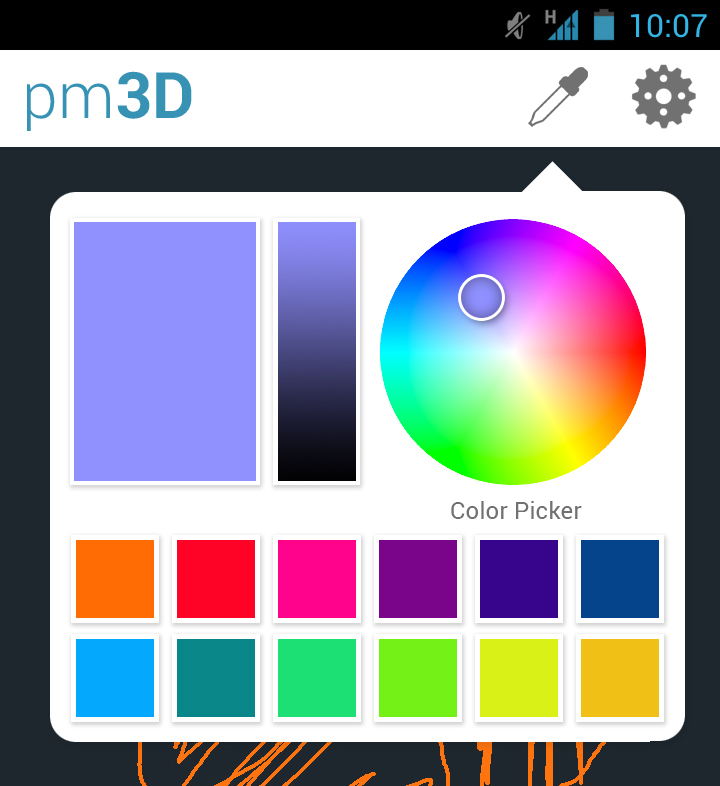
\includegraphics[width=\columnwidth]{colorpicker.jpg}
  \caption{When the user selects the eyedropper option in the Action Bar, the user is presented with a popup interface to select a color they wish to draw with.}
  \label{fig:colorpicker}
}
\end{figure}

%There are two screens in the program; main screen and settings screen. When
%the program opens, the user sees the main interface with which she can start
%drawing immediately by simply tapping the screen. There is an action bar at
%the top of the screen with two buttons. The first button, indicated by an
%eyedropper icon, enables the user to select a color from a default palette or
%pick another color using the color picker. Users can also see the selected
%color at the bottom of the screen while in drawing mode. They can stop drawing
%at any time and look at their drawing, using swipe and pinch gestures to orbit
%or zoom in view mode.

%Second button, indicated by a gear, is a link to the settings page. In this
%page, users can choose to toggle the usage of the camera and gyroscope or
%calibrate the accelerometer. Users can also see developer info and a link to
%the GitHub repository page of the project. There also options to save the
%current drawing, clear the screen, load another drawing, or share the current
%drawing on social networks.

\pagebreak

\section{Technology \& Implementation}

Since PaintMobile3D is an Android application, we naturally have made heavy
use of the Android API. Sensor data is acquired using from callbacks that are
made available by the Android operating system. In order to draw the points
onto the display for the user to see, we have made use of the OpenGL ES
library that is also provided by the Android API. While the accelerometer and
gyroscope provide directly applicable information straight from the sensor,
the data from the camera requires additional manipulation in order to make it
useful. For this, we are using the OpenCV implementation for Android, called
OpenCV4Android, to provide computer vision functionality, such as feature
extraction and motion tracking. After this data has been processed, it can
then be used by our localization algorithms. Some of the calculations needed
to perform localization for our application are computationally taxing. Since
the application is designed to run on a mobile device that has limited battery
power, we need to make these computations as efficient as possible. To do
this, we are using the Android NDK (Native Development Kit) to provide us with
direct access to the CPU using native code, instead of the managed environment
provided by Android's Dalvik Virtual Machine.

\section{Potential Applications}

PaintMobile3D is an application that is designed simply for user entertainment. However, additional work could add
considerable value. For example, if the phone is connected to a computer with a project, it's possible to draw in front of an audience,
allowing one to use PaintMobile3D as a virtual whiteboard. This could be improved further by allowing the importation of
3D models, which could be annotated live. These could be used for any number of purposes, from teaching to planning military tactics.

The motion tracking technology is valuable in itself for any number of tasks. Games are an obvious application. Using the phone as a
portal into a virtual world could be done by changing the camera position with the phone's position. With some calibration, using a
phone for measurement is possible by tracking the distance the phone travels.


\section{Acknowledgements}

We would like to acknowledge:

\begin{itemize}
\item
University of Nevada, Reno
\item
CHI Conference
\item
ACM
\item
Google
\end{itemize}

\balance

\bibliographystyle{acm-sigchi}
\bibliography{references}

\end{document}
